\documentclass[11pt]{article}

\usepackage{amsmath}
\usepackage{amsfonts} % to include additional math. characters such as R
\usepackage{graphicx} % to include images
\usepackage{hyperref} % to be able to click on references
\usepackage{multirow} % to merge cells in tabular env. vertically
\usepackage{subcaption} % for subfigures and +
\usepackage{longtable} % to have table that extends over multiple pages
\usepackage{lipsum}
\usepackage[left=2cm, right=2cm, bottom=3cm, top=3cm]{geometry}

\graphicspath{ {./Images/model_validation} }
\title{Cancer Immunotherapy - Planning Report}
\author{Alexandre Y. Péré }
\date{\today}

% What does not count: title page, table of content, abstract, acknowledg.
% tables and figures, appendices, captions, nomenclature and biblio.
% So what counts: section pure content
\begin{document}
\begin{titlepage}
    \newcommand{\HRule}{\rule{\linewidth}{0.5mm}}
    \begin{center}
        \HRule \\[0.4cm]
    { \huge \bfseries Cancer Immunotherapy: Planning Report \\[0.15cm] }
    Supervisors: Professor Reiko Tanaka, Doctor Tara Hameed 
    \\[0.4cm]
    \HRule \\[0.5cm]
    Alexandre Yann Péré \\[0.1cm]
    CID: 01938104  \\[0.1cm]
    \today \\ [0.1cm]
    \end{center}
\end{titlepage}

\tableofcontents


% Repartition of word count (total 4,000)
%
% Project specification (300)
% Litt Review (1,200-1,500)
% Schedule (500)
% Evaluation (300)
% Prelim Results (1,000)
% total=3,000

% QUESTIONS FOR TARA
% 1) What's the difference between GA validation and Bayesian validation??
\pagebreak 
\section{Project Specification}
% This section should state clearly what the project is intended to deliver. It should contain the AIMS, OBJECTIVES and HYPOTHESES of your work.

% Questions/comment: 
% - Should include "optimisation of treament for CR" in aims?

\par The aim of the cancer immunotherapy project is to use computational models to improve our understanding of the immune mechanisms behind the CBD-IL-12 immunotherapy, utlimately to characterise the responder profile for the treatment.\\[8pt]
\textbf{Objective 1:} validate the computational model of the immune response developed by previous researchers, and make modifications if necessary \\ 
\textbf{Objective 2:} identify key biological factors in mice that determine the outcome of the treatment, along with the corresponding threshold that separates CR from non-CR \\ 
\textbf{Objective 3:} associate each key factor to a corresponding biomarkers in mice\\ 
\textbf{Objective 4:} \textit{(potential!)}  understand how the boundary between CR and non-CR depends on the treatment characteristics (number and frequency of doses, combination with other treaments, etc.)

\section{Ethical Analysis}
The project's ethical foundation rests upon several crucial pillars. Scientific integrity is paramount, underlining the adherence to rigorous methodologies and transparent reporting of findings derived from animal tests on mice for cancer treatment. The project upholds scientific collegiality, fostering collaboration and open dialogue within the scientific community, enabling the exchange of insights and methodologies to advance cancer immunotherapy.

Regarding the subjects and specimens used, the project prioritizes the protection of human subjects by using animal models for initial testing, aiming to minimise potential risks to human health. This approach ensures stringent safety assessments and efficacy evaluations before any human trials. Animal welfare remains a cornerstone, demanding meticulous care and ethical considerations in handling and testing procedures, striving to minimise discomfort and stress for the animal subjects involved.

In the broader context of social responsibility, the implications of this work are profound. The potential to advance cancer immunotherapy represents a significant stride toward addressing a critical health concern, holding promise for enhancing treatment outcomes and potentially saving human lives. The long-term effects signify a potential shift in cancer treatment paradigms, ushering in more targeted and effective therapies.

The impact extends beyond the scientific realm, influencing colleagues, the College, society, and the environment. Collaborators and peers benefit from shared knowledge and advancements, fostering a culture of innovation and progress. The College gains recognition for its commitment to pioneering research with potential life-altering implications. Societal implications are vast, offering hope for improved cancer treatment and outcomes, positively affecting countless lives. Additionally, the project emphasizes environmental responsibility by ensuring ethical use of resources and minimising any potential ecological impact associated with research activities.

Ultimately, this project embodies a commitment to ethical, responsible, and impactful scientific research, rooted in principles of integrity, collegiality, human subject protection, animal welfare, social responsibility, and environmental mindfulness.
\pagebreak
\section{Background}\label{sec:background}
% Summarise the key findings from a range of published sources that you have used to identify research gaps, shape your aims and objectives, and justify the decisions you are making in your methodology. The text should be clear, with use of figures (with attribution) if helpful to the explanation.

\iffalse % Multiline comment 
Plan:
I - Introduce state of therapies, unmet needs, ie explain why the project makes sense in the pharma industry
II - Introduce in more details result of Jun Ishihara on the CBD-IL-12 specifically
III - Explain why computational modelling approach make sense (cite similar analysis for example).
IV - Justify the methodology I suppose? So cite Bayesian Workflow from Gelman. Also justify why sens. analysis makes sense to reduce dimensionality, etc. Maybe mention that obj. 1 and 2 are concurrent, meaning that I have to work on them at the same time.
V - ?? This should be enough
\fi

\quad Cancer is a large class of diseases that is the second leading cause of death in the United-State \cite{nchs}. One of its distinctive characteristics is that it can escape the human immune system, making it very hard to detect and fight naturally \cite{EvasionMech}. Traditional methods, such as chemotherapy or surgery, rely on using destructive external agents to kill the cancerous cells. However, introducing foreign agents in the body often results in heavy side effects [cite!]. This urged oncology research to try develop less ... [intrusive?] methods, which eventually led to the discovery of immuno-oncology treatments (or immunotherapies) in 2010 [cite]. 

~
\par While all cancer immunotherapies focus on using the natural immune system to fight against cancer, many different variations exist. The specific therapy of concern in this project is a combination of cytokine-based treatments and immune checkpoint inhibitors. Before explaing its mechanisms of action in more details, we will review the general principles behind the two aforementionned types of immunotherapy. In both case, a specific type of T-lymphocyte -- the CD8$^+$ T-cells -- is the central actor \cite{ReviewCPI}. CD8$^+$ differentiate itself from other T-cells through the expression of the membrane receptor CD8, and its main function is to directly carry out cytotoxic activity (i.e. killing the malignant cells) after detecting tumoural antigen~\cite{cd8Effects}.
\par Cytokine-based therapies seek to make use of specific cytokines -- small proteins that act as signalling molecules during the immune response -- to control tumour growth \cite{ioDef}. One of the most promising cytokine thus far is the interleukin-12 (IL-12), that was shown to have very potent antitumour effects, including introducing long-term memory in CD8$^+$ T-cells~\cite{il12IsCool}. More specifically, IL-12 action mechanisms follow three pathways. First, it activates the production of tumour-infiltrating cytotoxic cells, mainly CD8$^+$~\cite{cd8FirstWay}. Secondly, it is a pleiotropic molecule, meaning that it results in the release of numerous cytokines throughout the immune response~\cite{il12CytokineStorm}. One particular molecule released during this cytokine storm is the interferon-$\gamma$ (IFN$\gamma$). IFN$\gamma$ also plays a dominant role, as not only does it have anti-angiogenesis effect~\cite{ifngAngiogenesis}, thus limiting cancer growth; but it also stimulate production Natural Killer cells \cite{ifngNKProd} (another type of cytotoxic cells capable of attacking tumours) and upregulate antigen-presenting pathways within tumour cells \cite{ifngAntigenExposure}. Finally, IFN$\gamma$ facilitates T-cell proliferation by reducing negative regulatory pathways that lead to immunosuppression. It  increases the duration of IFN$\gamma$ effects by reducing IFN$\gamma$-induced apoptosis, and inhibts the effect of the immune checkpoint PD-1, similarly to chekpoint inhibitors (CPI) treatments \cite{reducImmunoSuppression}. The more details mode of action is described in the following paragraph. [maybe need to mention trAEs? and poor performance so far...]
\par To understand checkpoint inhibition, we must first review in more detail the negative regulatory pathways of T-cell activity. The most potent pathway involves checkpoint molecules, either Cytotoxic T-lymphocyte antigen 4 (CTLA4) or programmed cell death 1 (PD1) \cite{cpiProof}. Both molecules are membrane protein receptors that act with some delay to exhaust T-cell functions after they are activated by antigen-presenting cells (APC). Through in-vivo experiments, their main purpose was shown to be prevention of autoimmunity \cite{PD1Autoimmune}. However, in the presence of cancerous tissues, their normal function are deregulated, resulting in abnormal behaviour and immunosuppression [need more details about PD1 and CTLA4?]. The main difference between CTLA4 and PD1 is the type of tissue they regulate: CTLA4 tempers activation locally in lymphoid organs, whereas PD1 acts in peripheral tissues \cite{PDvsCTLA}. The idea behind CPI immunotherapies is to precisely block the immunosuppressive pathways of CTLA4 and PD1, to shift to tumoural microenvironment toward being immunologicaly active. Clinical trials demonstrated positive results in several types of cancers [cite], but performed poorly against immunologically cold tumours, i.e. tumour that do not normally elicit a strong immune response (they escape the immune system very effectively), such as melanoma [cite].  

% In contrast with the traditional therapies mentioned above, it relies on using human’s own defence mechanisms to fight against the cancerous cells. It has quickly drawn attention as an option that has the potential to induce complete remission -- meaning that there is no more evidence of cancer, although cancer recurrence is still possible -- with little treatment-related adverse events (trAEs). However, while being a promising avenue,  the CR rate for current drugs is still generally low, less than 10\% \cite{ott}. This shows that current products are not optimal yet and new paths have to be explored. More patient could benefit from these treatments if we could understand why some patients respond to the treatment while some do not.

~ % Section about CBD-IL-12 specifically
\par Recent endeavours in this field of immunotherapies led to the development by Mansurov, Ishihara et al. of a new molecule -- CBD-IL-12 -- that demonstrated promising results to treat melanoma \cite{cbdil12}. The CBD-IL-12  molecule consists of a collagen-binding protein (or collagen-binding domain, CBD) that is fused onto a IL-12 cytokine. The new molecule hence only accumulates in collagen-rich regions, as it is the main component of cancerous microenvironment \cite{collagenInCancer}. This is results in an enhanced delivery method that can achive high concentration of IL-12 specifically in cancerous microenvironment. In mice tumour-models, this novel molecule achieved a CR rate of up to 67\% for melanoma, and 87\% for breast cancer when combined with CPI drugs (a mix of both anti-PD1 and anti-CTLA4). While these results are very encouraging, it was also shown in the same study that they are hardly reproducible, as they depend on a myriad of factor through still unkown mechanisms, such as the tumour volume at injection, quantity injected, etc. This motivates us to study this specific immunotherapy more carefully, as a better understanding of the principles governing the immune response seems necessary to optimise this new treatment.

~ % Section about the state of the project when I took it 
\par To this end, T. Miyano (2019) proposed an initial mechanistic model based on Delay-Differential Equations (DDEs), parameterised by 21 parameters representing various relevant biological factors of a given mouse, such as the tumour growth rate or the degradation rate of IFN$\gamma$ \cite{takuya} [should I put the model here or in the appendix]:
\begin{align*}
    \dot{g}(t) &= k_1 + k_2 [d_{CBD}(t) + d_{12}(t)] - d_1g(t) \\ 
    \dot{c}(t,t-t_d) &= k_3 + k_4g(t-t_d)-d_2c(t) \\ 
    \dot{p}(t) &= k_5 - [d_3 + d_4g(t)]p(t) \\ 
    \dot{v}_l(t) &= k_6\left[1 - \frac{v(t)}{v_{max}} \right]v_l(t) - \left[d_5 + \frac{\frac{d_6c(t)}{1+s_1p(t)(1-d_{CPI}(t))}+d_7g(t)}{1+s_2v(t)}\right]v_l(t)\\
    \dot{v}_d(t) &= \left[d_5 + \frac{\frac{d_6c(t)}{1+s_1p(t)(1-d_{CPI}(t))}+d_7g(t)}{1+s_2v(t)}\right]v_l(t) - d_8 v_d(t)
\end{align*}
This model is based on the main mechanisms/pathways that control tumour growth: IFNg, CD8+ and PD-1. This is motivated by the findings by Mansurov et al. \cite{cbdil12} and well as private discussions with co-author Ishihara. This was further investigated by C. Hines, who showed that the model could successfuly reproduce experimental data by using a Genetic Algorithm for parameter fitting \cite{christian1}. However, C. Hines also demonstrated in a subsequent analysis that the model was conflicting with findings from the biologists, as not only as the model was missing a key feedback loop \cite{christian2}, but also since the model's behaviour is largely insensitive to the initial tumour volume and treatment characteristics \cite{christian1}. These results motivate us to further investigate the model, and potentially refine it if necessary. 

~ % Section about the choice of computational tools
\par Regarding the choice of computational tools necessary for this project, a study by Rozenbaum et al. (2019) about popoulation inference through Bayesian modelling played a large role. In this study, the authors resorted to hierarchical Bayesian. 

demonstrated that hierarchical Bayesian inference was an effective approach to explain data heterogeneity at the population level \cite{rosenbaum}. [Add more details, esp. related to the findings]. This confirms C. Hines \cite{christian2} who also advocated for a Bayesian approach of the problem. Amonst the other computational tools required for the analysis, sensitivity analysis is of particular interest, as shown by \cite[text]{sens_review} 

~ % Section about the biomarkers identification step
\par A paragraph for litt review about cancer biomarker identification and already existing ones.

% MoHowever, in the same study this success rate was shown to be highly dependent on a number of factors such as the dose, combination with other treatments, initial tumour volume, etc. As the mechanisms of action of CBD-IL-12 are still unclear, it is difficult to predict the outcome of a specific treatment, or to design an effective treatment, for a given patient. This hence motivates us to study this specific molecule more carefully, as a better understanding fo the main principles governing the immune response seems necessary to maximise and optimise this new treatment.
\par  

\section{Implementation Plan}\label{sec:plan}
% Question for Tara: what if the revised mechanistic model does not capture the dual outcome that is initially present? Does that mean the model is wrong, or that the dual outcome is not exactly accurate?
In light of the knowledge gathered through the litterature review presented above, the proposed plan to fulfill the 4 (3?) objectives is as follows.\\[12pt]
%
\noindent\textbf{Task 1.1 -- Evaluation of the initial model (already completed)}\\
First we familiarise with the initial mechanistic model of the immune response developped by Takuya. This includes numerical stability/bifurcation analysis, sensitivity analysis to find the boundary between CR and non-CR in parameter space. This step is necessary to understand to general design principles that guide the development of a mechanistic model, and can potentially reveal some of the model weaknesses that need to be addressed. The sensitivity analysis is also key to reduce the dimensionality of the problem, since the model is otherwise too large and would result in intractable computations.\\[12pt]
%
\noindent\textbf{Task 1.2 -- Non-hierarchical model validation (already completed)}\\ 
The second step is to verify that the model can be used to perform Bayesian inference, as this will be at the core of the analysis. To do so, we will follow the the procedure highlighted by Gelman et al, 2020, in their \textit{Bayesian Workflow} paper \cite{gelman2020bayesian}. Essentially, the validation consists of three main steps: prior predictive check, fake data check and posterior predictive check. For each step, the paper provides a list of potential methods to improve the model if it fails the corresponding test. The Bayesian analysis relies on using a hierarchical model, however we propose to first validate simpler, non-hierarchical model twice: with complete- and no-pooling. [Explain why! maybe cite as well]\\[12pt]
%
\noindent\textbf{Task 1.2a (fall-back 1) -- Validate using Approximate Bayesian Computation (1-2 month)}\\ 
The above validation procedure might fail in two ways : either the model produces wrong results, or it cannot even produce results (for example, the MCMC chains cannot explore the posterior distribution well). In case the latter happen, it would be due to the high complexity of the likelihood function (the mechanistic model of the immune response), a set set of five Delayed Differential Equations that cannot be solved analytically. One way to reduce this complexity would be to use Approximate Bayesian Computation (ABC), which is a likelihood-free framework \cite{ABCtuber}. This approach would enable us to prevent the inference from running into convergence problems, at the cost of slightly less exact results. \\[12pt]
%
\noindent\textbf{Task 1.2b (fall-back 2) -- Validate using simplified likelihood function (2-3 months)}\\
As suggested in the \textit{Bayesian Workflow} paper, another method to solve convergence issues would be to simplify the likelihood function, for example by using Ordinary Differential Equations instead of DDEs. This is an alternative to ABC, and would require more time to implement as it needs to completely review the tumour model. However, contrary to ABC, it is still a traditional Bayesian inference and hence does not results in approxmation errors that can have a non-negligible impact, as highlighted by Robert et al, 2011 \cite{ABCerror}\\[12pt] 
%
\noindent\textbf{Task 1.2c (fall-back 3) -- Modify the model (3 months)} [need refo.]\\ 
The two fall-backs described above are mostly usefull to address convergence issues, but may not help much if the model produces wrong results. In this case, the most sensible approach would be to modify the Bayesian model (either the priors or the likelihood, depending on which test was not passed). Using litterature about cancer immunology will be key, as is especially suggests that a key feedback loop is missing in the current model [cite!!]. During this process, it is likely that we will need to use a Genetic Algorithm for parameter fitting. This is especially useful to test that the mechanistic model can reproduce the data, without having to resort to a full Bayesian inference, where many additional elements interact together. \\[12pt] 
%
\noindent\textbf{Task 1.3 -- Validation of the hierarchical model (??)}\\ 
Once two component of the hierarchical model are validated (the no-pooling and complete-pollingn models), it is necessary to validate the hierarchical model itself. We will follow the same procedure (include the fall-backs) as for the non-hierarchical models. [anything else to mention here?]\\[12pt]
%
\noindent\textbf{Task 2.1 -- Extensive numerial analysis of the compuational model}\\ 
This is the first set of analysis we plan to do on the validated model. First we perform a sensitivity analysis, using the eFAST method as justified in Section~\ref{sec:background}. This is necessary to know if a given parameter should be set as a free or fixed parameter. This makes practical implementation of the subsequent analysis possible, while minimising the error we introduce. Then, we plan to perform a bifurcation analysis to evaluate the boundary surface in parameter space that separates CR from non-CR. We expect a grid-search bifurcation to be sufficient, since only trans-critical bifurcation can happen (Hopf would not make biological sense... ?). \\[12pt]
%
\noindent\textbf{Task 2.1a (fall-back 1) -- ?}\\ 
What happens if the model does not capture the bifurcation behaviour? Does it mean that the model is wrong? \\[12pt]
%
\noindent\textbf{Task 2.2 -- Full Bayesian Inference}\\ 
I do not really know what to say here.\\[12pt]
%
\noindent\textbf{Task 3 -- Biomarker Identification}\\ 
Having identified the key parameters that encode the outcome heterogeneity along with their bifurcation point, we will link each of them to a corresponding mouse biomarker. We suspect that the exact methodology will depend on which parameters are selected for this step, but we propose to follow to general methodology for biomarkers identification presented in Section~\ref{sec:background}, relying on genomic data and statistical tools. We will also make use of the already-existing litterature about cancer biomarkers that measure potential response to therapy. \\[11pt]
%
\noindent\textbf{Task 3.a (fall-back 1) -- Collect genomic data}\\ 
If genomic data is not available, means that we will have to collect it first. It is likely that the project will thus not be finishable, so will only be able to design computational/theoretical framework for biomarker identification without practical implementation.  

\section{Risk Register}
The main risks are : 

\begin{longtable}{|p{3.5cm}|p{2.5cm}|p{4.5cm}|p{5cm}|}
    \hline
    \textbf{Risk} & \textbf{Likelihood} & \textbf{Impact} & \textbf{Mitigation Strategy}\\
    \hline
    \endfirsthead
    \hline
    \textbf{Risk} & \textbf{Likelihood} & \textbf{Impact} & \textbf{Mitigatio Strategy}\\
    \hline
    \endhead
    \hline
    \multicolumn{4}{|r|}{\textit{Continued on next page}} \\
    \hline
    \endfoot
    \hline
\endlastfoot
        \hline
        not finishing \\ the project & dedes & 3 & 4 \\ \hline 
    \caption{Table of the different risks associated with the project's objectives}
    \label{tbl:hyperparams}
\end{longtable}
\section{Evaluation}
Below we present a list of the key components of the cancer immunotherapy project, along with a way to verify that they function correctly. The Bayesian encompasses the mechanistic model, as the likelihood function. \\[11pt]
%
\textit{Mechanistic Model}\\[3pt] % TODO: appendix ??
The mechanistic model is the core element of the project. Its `quality'' can be asessed by two criteria: it should be able to reproduce the data obtained in the lab by Dr. Ishihara (see Appendix), and it should make ``biological sense''. To assess the former, we propose to use the standard method of parameter fitting through a Genetic Algorithm (GA), which has already been used in the past for this purpose \cite{christian2}. This enables us to find a parameterisation of the model that leads to the best simulation, along with the Mean-Squared Error to the true data. This metric can be used to validate that the model can produce data close enough to the experimental time series. To assess the second criteria, we will use a sensitivity analysis (namely, the eFAST method [should justify?]). It enables us to check that the model is sensitive to the same quantity as shown in the lab [wording is terrible here, need to rephrase], for example to the treatment specification or to the initial tumour volume, which is not the case for the current one. [need to describe experiments more?]\\[11pt]
%
\textit{Bayesian Model}\\[3pt]
To validate the Bayesian model, which is an extension of the mechanistic model, we will follow the Bayesian Workflow procedure, as explained on Section~\ref{sec:plan}. Describe here with more detail, but nothing else to be explained.\\[11pt]
%
\iffalse
\textit{Biomarkers}\\[3pt]
lorem ipsum\\[11pt]
%
\fi
\textit{Responder Profile}\\[3pt]
lorem ipsum

\section{Preliminary Results}
\subsection{Sensitivity Analysis}
In order to restrict the parameter space for subsequent analysis, and also to understand to main mechanisms behind the immune response, we performed a eFAST sensitivity analysis on the initial DDE model developed by T. Miyano. Results are shown in Fig.~\ref{fig:efast}. As can be seen, we can that the main effect indices (in blue) are always negligible compared to the interaction indices (orange). Accordin to a study by Vazquez-Cruz et al. (2012), this is a typical sign of non-identifiability \cite{tomgro} that will significantly hinder Bayesian inference. Additionally, results indicate that the treatment characteristics (labelled \verb+tem+, \verb+td+ and \verb+ti+) have almost no impact on the treatment outcome, which is conflicting with the results experimentally obtained in the CBD-IL-12 study \cite{cbdil12}. 

\begin{figure}[!ht]
    \centering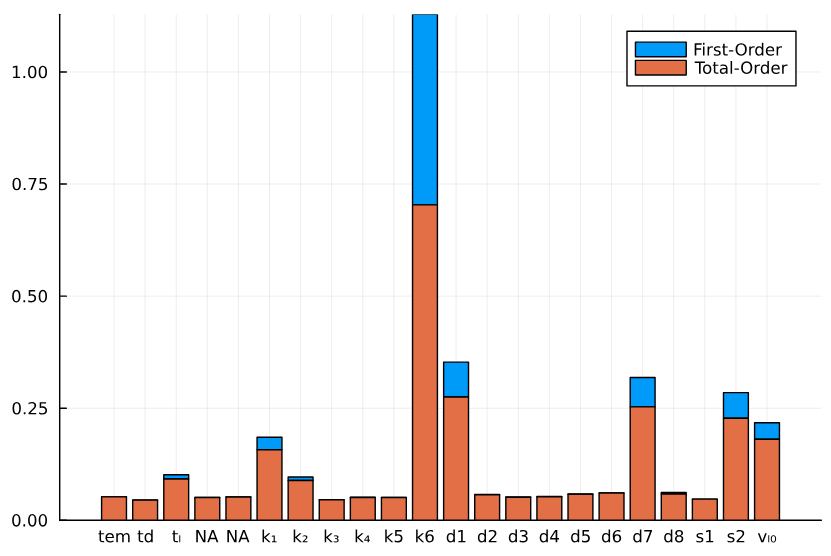
\includegraphics[scale=0.4]{Images/batch2/eFAST_old.png}
    \caption{Results of the eFAST sensitivity analysis on the initial model}
    \label{fig:efast}
\end{figure}
\subsection{Numerical Stability Analysis}

\subsection{Bayesian Model Validation}

\subsection{Switchng to Approximate Bayesian Computation}

\newpage 
\clearpage
\newpage

\addcontentsline{toc}{section}{References}
\bibliographystyle{unsrt}
\bibliography{biblio}


\end{document} % This is the end of the document
